%!TeX spellcheck = en-US
%!TEX root = ../hw4_report.tex
Consider the PDE
\begin{equation}
\begin{aligned}
\Delta u+g(x,y)u &= f(x,y),\text{ for }x,y\in\Omega,\\
u(x,y) & = 0,\text{ for }x,y\in\partial\Omega,
\end{aligned}
\end{equation}
where $\Omega$ is the unit square.
\subsection*{(a)}
\emph{Derive the 2nd order finite-difference discretization for the grid $x_i = hi, i = 1,\dots,m,y_j = hj,j = 1,\dots,m$ and $h = 1/(m+1)$. Also, derive matrices such that the discretizatioin can be expressed as
\begin{equation}\label{lyapPDE}
D_{xx}U+UD_{xx}+G\circ U = F,
\end{equation}
where $U_{i,j} \approx u(x_i,y_j)$. }

Using a 2nd order approximation of the second derivatives
\begin{equation}
\frac{\partial^2 f}{\partial x^2} = \frac{f(x+h)-2f(x)+f(x-h)}{h^2}
\end{equation}
and similarly for $\frac{\partial^2 f}{\partial y^2}$, we can approximate the laplacian by the five point stencil
\begin{equation}
\Delta u_{i,j} \approx \frac{u_{i-1,j}-4u_{i,j}+u_{i+1,j}+u_{i,j-1}+u_{i,j+1}}{h^2},
\end{equation}
for $i = 1,2,\dots,m$ and $j = 1,2,\dots,m$.
From the boundary condition, we have
\begin{equation}
u_{0,j} = u_{m+1,j}=u_{i,0} = u_{m+1,0} = 0.
\end{equation}
The structure for the Laplace operator alone is thus the $m^2\times m^2$ matrix
\begin{equation}\label{tridiag}
\begin{bmatrix}
T &I &0 &\dots& 0\\
I & T& I & \dots \\
\vdots &\vdots& \vdots &\vdots& \vdots\\
0 & 0 & 0 &I& T
\end{bmatrix}
\end{equation}
with $T$ being the $m\times m$ matrix with $-4$ on the diagonal, 1 on the sub- and super-diagonals and zero otherwise.
The entire system for the PDE can be written on the form $Au = b$, where $A$ has the same structure as the matrix in \eqref{tridiag}, but where the diagonal is given by matrices $B_1,B_2,\dots, B_m$, where $B_j = T+h^2\cdot GG_j$, with $GG_j$ having values only on the main diagonal taking the values $g(x_i,y_j)$, $i=1,\dots,m$. The right hand side vector $b$ is given by
\begin{equation}
b = h^2
\begin{bmatrix}
f(x_i,y_1)\\
f(x_i,y_2)\\
\vdots\\
f(x_i,y_m)
\end{bmatrix}.
\end{equation}


Observe that this is the vectorized form of the equation \eqref{lyapPDE}, where
$D_{xx}$ is a $m\times m$ matrix with -2 on the main diagonal and -1 on the sub- and superdiagonals, $G =h^2\cdot g(x_i,y_j)$ and $F = h^2\cdot f(x_i,y_j)$.
\subsection*{(b)}
\emph{Derive explicit expressions for the eigenvalues of $I\otimes D_{xx}+D_{xx}\otimes I$ in the limit $m\to\infty$ and show that the matrix $I\otimes D_{xx}+D_{xx}\otimes I$ is non-singular in the limit.}

First, we identify that the matrix $I\otimes D_{xx}+D_{xx}\otimes I$ is the finite difference approximation of the laplace operator. In the limit $m\to\infty$, the approximation approaches the continuous laplace operator. Therefore, we seek eigenvalues
\begin{equation}
\Delta u = \lambda u.
\end{equation}
Writing $u$ as $u(x,y) = X(x)Y(y)$, we get the equation
\begin{equation}
X''+Y'' = \lambda XY \Leftrightarrow \frac{X''}{X}+\frac{Y''}{Y} = \lambda,
\end{equation}
enforcing that for some constants $\alpha$ and $\beta$,
\begin{equation}
X''=\alpha X\text{ and }Y'' = \beta Y.
\end{equation}
Solving these equations along with the homogeneous boundary conditions, we obtain that
\begin{equation}
\lambda = (k\pi)^2+(l\pi)^2,\quad k,l = 1,2,3,...
\end{equation}
The equations for $X(x)$ and $Y(y)$ have no nontrivial solutions for $\lambda =0$ and thus it can be concluded that the matrix is non-singular.
\subsection*{(c)}
Letting
\begin{equation}
g(x,y) = \alpha\sqrt{(x-\frac{1}{2})^2+(y-\frac{1}{2})^2}
\end{equation}
and $f(x,y)= |x-y|$, we do the following (comparing solution techniques and timing results):
\begin{enumerate}
\item Let $\alpha = 0$ and solve the sparse linear system $Au = b$ using $\backslash$.
\item We compare the above with solving the equation using the matlab command \texttt{lyap}.
\item Let $\alpha = 1$ and solve with $\backslash$

\begin{figure}[h]
    \centering
    \begin{subfigure}[t]{0.48\textwidth}
        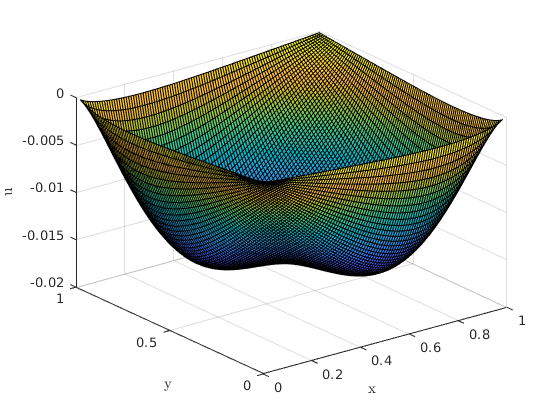
\includegraphics[width=\textwidth]{u12a.png}
		\caption{Solution task 12: 1. and 2. computed with $m=100$.}
    \end{subfigure}
    \begin{subfigure}[t]{0.48\textwidth}
        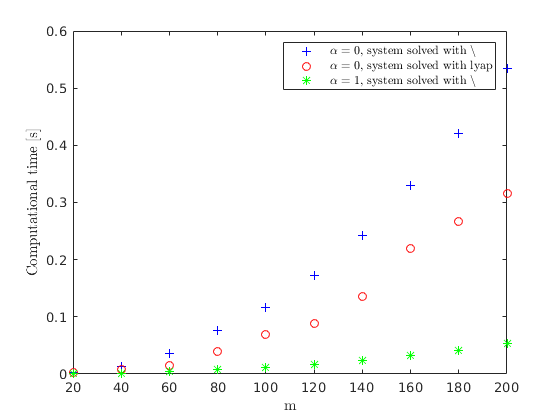
\includegraphics[width=\textwidth]{time12.png}
        \caption{Timeing results for tasks 12: 1-3.}
        \label{timeab}
    \end{subfigure}
    \caption{Tasks 1-3}
\end{figure}


Computing the difference between the solutions in task 12 1) and 2) with $m=100$ yiels $\|U_1-U_2\| \approx 1.37\times 10^{-12}$ and the average time when solving the system 10 times for different matrix sizes and choices for $\alpha$ is found in Figure \ref{timeab}. It can therefore be concluded that it is significantly faster to solve the matrix equation using \texttt{lyap} instead of solving the linear system using $\backslash$ and also that the system faster can be solved with $\backslash$ if $\alpha=1$ than if $\alpha = 0$.
\item Again, let $\alpha = 1$, but use instead \texttt{gmres} to solve the system.

We conclude that gmres fails to converge to desired tolerance within a reasonable number of iterations. Setting $m=100$, the relative residual after RESTART*MAXIT$=20\times 10$ iterations is 0.0886.
\item Using $\alpha = 1$ and \texttt{gmres}, use \texttt{lyap} as a left pre-conditioner.

A left preconditioner is a matrix $M$ modyfing  the system $Au = b$ such that the new system to solve is $M^{-1}Au = M^{-1}b$. A function computing the action of an inverted preconditioner matrix applied to a vector $z$ can be formed using \texttt{lyap}$(T,-Z*h^2)$, where $Z=$\texttt{reshape(z,m,m)} and where the result from the \texttt{lyap} command is reshaped to a vector of size $m^2\times 1$. Solving the system using $m=100$, gmres and the described left-preconditioner, we can compute the norm $\|U_{\text{backslash}}-U_{\text{gmres with precond}}\| \approx 1.50\times 10^{-9}$.

\item Using $\alpha = 0.1$ and \texttt{gmres}, use \texttt{lyap} as a left pre-conditioner.

We compare the computational time for an average of 10 solves using $\backslash$ and $\alpha = 1$, pre-conditioned \texttt{gmres} and $\alpha=1$ and pre-conditioned \texttt{gmres} and $\alpha = 0.1$. The result is visualised in Figure \ref{time12_2}. It can be concluded that the pre-conditioned \texttt{gmres} performes better in terms of computation time for $\alpha = 0.1$ than for $\alpha = 1$. It should also be noted that solving with backslash is faster than using gmres, which might be due to how we have chosen to construct the preconditioner-function.
\end{enumerate}
\begin{figure}[h!]
\centering
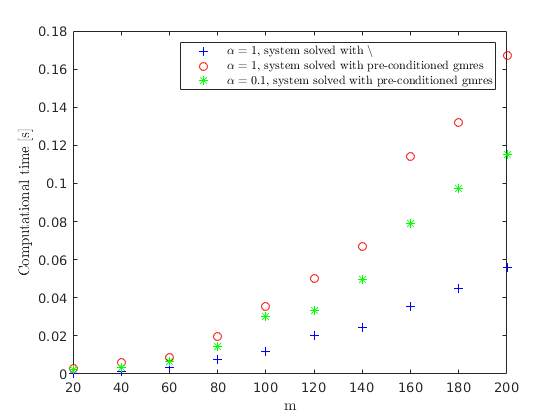
\includegraphics[scale=0.6]{time_gmres.png}
\caption{Timing results comparing the preconditioned gmres for different $\alpha$ and also comparing to results using $\backslash$.}
\label{time12_2}
\end{figure}

\subsection*{(d)}
\emph{Explain the performance in (c) of the the preconditioned gmres.
}
Consider $A-E$ to be the matrix $A$ obtained by choosing $\alpha = 0$. Then, from the hint in the lecture notes,
\begin{equation}
(A-E)^{-1} = A^{-1}-A^{-1}EA^{-1}+\mathcal O(\|E\|^2),
\end{equation}
for sufficiently small $\|E\|$. The matrix $E$ is diagonal, having only the values $h^2\cdot g(x_i,y_j)$ on the diagonal ordered columnwise, and therefore, $\|E\|_2 = h^2\cdot \max(g(x_i,y_2))<h^2\cdot\alpha \sqrt{2}/2$. Thus, using the solution from the lyap command (with $\alpha = 0$) as a pre-conditioner, the inverse of the preconditioner $M=A-E$ is very close to being the inverse of the matrix $A$ where e.g. $\alpha = 0.1$. The consequence is clearly that gmres converges in few iterations as the product $(A-E)^{-1}A\approx I$.

\subsection*{(e)}
\emph{Suppose all elements of the matrix $G$ are zero except $G_{m/4,m/2} = 1/h$, where $m\in 4\mathbb Z$. Solve the equation efficiently by using the \texttt{lyap} command.}

We consider the problem as a rank-one modification and use the Sherman-Morrison-Woodbury formula, stating that if $A$ is an invertible square matrix and $u$, $v$ are column vectors of the same size, then $A+uv^T$ is invertible iff $1+v^TA^{-1}u\neq 0$. The inverse is given by
\begin{equation}
(A+uv^T)^{-1} = A^{-1}-\frac{A^{-1}uv^TA^{-1}}{1+v^TA^{-1}u}.
\end{equation}
%Using $u = e_{m/4}$ and $v  = (1/h)e_{m/2}$, we can then compute
We want to solve a large and sparse linear system of the form
\begin{equation}\label{orig}
(A+\tilde{G})x = b,
\end{equation}
where $\tilde{G}$ is the sparse matrix putting the values of the matrix G on the diagal columnwise.
Using that $\tilde{G} = uv^T$, we obtain
\begin{equation}\label{woodbury}
(A+\tilde{G})x = b\quad\Leftrightarrow\quad (A+uv^T)x = b
\quad\Leftrightarrow x=(A-uv^T)^{-1}b.
\end{equation}
Now, applying the Sherman-Morrison-Woodbury formula, \eqref{woodbury} can be rewritten as
\begin{equation}
x=(A-uv^T)^{-1}b = A^{-1}b-\frac{A^{-1}uv^TA^{-1}b}{1+v^TA^{-1}u}.
\end{equation}
We identify that for the specified matrix $G$, $u =e_{(m/2-1)m+m/4}$ and $v = (1/h)\cdot e_{(m/2-1)m+m/4}$. The problem thus boils down to solving a lyapunov equation twice with different right hand sides and then vectorize the results. In pseudo-code, we compute
\begin{equation}
\begin{aligned}
&\alpha = \texttt{lyap}(T,-F);\\
&\alpha = \alpha(:);\\
&\beta = \texttt{lyap}(T,-e_{(m/2-1)m+m/4});\\
&\beta = \beta(:).
\end{aligned}
\end{equation}
Then,
\begin{equation}
x=(A-uv^T)^{-1}b  = \alpha -\frac{\beta(v^T\alpha)}{1+v^T\beta}.
\end{equation}

We compare with a naive approach solving \eqref{orig} using $\backslash$. Using $m=100$, the 2-norm difference between the solutions is $1.37\times 10^{-12}$.
